%!TEX root = ../main.tex
\documentclass[a4paper,oneside,12pt, class=Latex/Classes/PhDthesisPSnPDF, crop=false]{standalone}
\usepackage{setspace}
\begin{document}
\doublespacing
\chapter{A real-time search for Type Ia SNe with late-time CSM interaction in ZTF}
\label{chap:Real-time}
In chapters \ref{chap:DR2_search} and \ref{chap:pre-ZTF_search} I searched for late-time signals in old transients, with most results being found after the period of activity. Follow-up was only attempted for SN 2019ldf (photometric) and SN 2020alm (spectroscopic) in section \ref{Additional_tests}, but these provided no further signs of late-time CSM interaction. In order to understand more about the late-time signals that are recovered by binning the ZTF light curves, it is crucial to follow promising objects up using larger telescopes.

For this reason, I automate my pipeline to search a sample of SNe Ia observed by ZTF for currently active late-time signals using the latest observations. By doing this regularly, it is possible to find promising objects early and follow them up. My position as a student support astronomer at the Isaac Newton Group of Telescopes (ING) and Nordic Optical Telescope (NOT) proved to be extremely advantageous in obtaining time to observe targets using a 2.5 m telescope, but this time has very low priority. It proved to be crucial for quick follow-up of several objects that are presented in this chapter, especially SN 2020qxz (see section \ref{sec:SN2020qxz}).

This chapter is based on Terwel et al., (in prep.), which is currently being written and will be submitted to A\&A. The sample selection, data reduction, analysis and interpretation were performed by me. Where relevant, I have noted the specific parts that were carried out by collaborators. In section \ref{data} I present the sample used in the real-time search and explain where the latest observations come from. Section \ref{analysis} describes the automated pipeline, details the telescopes used in the follow-up campaign, and gives a short overview of the reduction. In section \ref{results} I describe the results for the promising objects that were found during the run of the real-time search. These are discussed in section \ref{discussion}, and I conclude in section \ref{conclusion}.


\section{Data}
\label{data}
To create a SN Ia sample to search for late-time CSM interaction in real time, I collect all spectroscopically classified SNe Ia in ZTF using the Fritz broker \citep{skyportal2019, Skyportal} and selected those objects that were first detected before 8 July 2023 (mjd 60133). Using this date cutoff ensures that all targets are over 100 days old at the start of the real-time search, and any new observations can be considered to be late-time observations of the SNe. This gives me a sample of 6\,914 SNe Ia. Using the \textsc{fpbot} package \citep{fpbot}\,\footnote{\url{https://github.com/simeonreusch/fpbot}} I construct the most up-to-date ZTF light curves for every object in my sample. ZTF uses difference imaging to remove constant sources from the science images and isolate the transient. Then, \textsc{fpbot} forces a PSF fit at a given location in the difference images to construct a light curve at that position spanning the entire survey.

As this sample contains all ZTF SNe Ia up until the first half of 2023, this naturally includes the entire ZTF SN Ia DR2 \citep[][Smith et al., in prep.]{DR2_Overview}, which have previously been examined for late-time signals in \citet{Terwel_2024_paper1}. 69 objects that were not available on Fritz when I made my sample have been excluded. However, as the latest data point used in \citet{Terwel_2024_paper1} is on 26 June 2022 (mjd 59756) I probe their SNe at later phases, and they could (have) become active after the time period examined by \citet{Terwel_2024_paper1}. Therefore, checking the same sample again could identify new late-time detections.

I aim to find late-time excesses while they are active, so the light curves have to be regularly updated with the latest observations. The ZTF survey is split into three parts: 40\% is a private partnership survey whose data I can access immediately after the observation and becomes publicly available after 18 months. 40\% is a public survey whose data is released every three months after a three-month proprietary, resulting in a three to six-month delay. The last 20\% is private Caltech time, whose data is released publicly after 18 months.

I use the binning method from \citet{Terwel_2024_paper1} to search for faint signals, binning observations over 100 days after the SN peak together in bins of 25, 50, 75, and 100 days. (see section~\ref{analysis}). The light curves do not have to be updated daily, as it will take several observations to push the detection limit deep enough to detect a faint signal in the latest bin. As the smallest bin size in the pipeline is 25 days, I aim to be able to create one additional bin each time an object is updated. I therefore split the sample into 28 lists and update the objects in one of these each day. This results in every object in the sample being checked and updated once every four weeks.

\section{Analysis}
\label{analysis}
Each time the light curves of the SNe Ia in my sample are queried and updated, they are run through the analysis pipeline from \citet{Terwel_2024_paper1}. This pipeline takes all observations at a given sky position and after pre-processing (including applying a baseline correction to correct for systematic offsets across the light curve, see e.g. \citealt{Yao_baseline_corr, Miller_baseline_corr}) and finding the SN peak, it will bin all observations in each band that are over 100 days after the SN peak in bins that have a size of 25, 50, 75, or 100 days. By doing so, the noise in the data is reduced, allowing to probe objects that are up to nearly a magnitude below the noise limit of single observations (m $\approx20.5$ mag) at the price of a reduction in the time sensitivity. This method is able to push the detection limit until the magnitude limit of the used reference images become the dominant source of uncertainty, which is around $\overline{\text{m}} \approx21.8$ mag for ZTF \citep{ref_uncert}.

When the pipeline detects a possible late-time signal, whether currently or previously active, the object is rechecked manually to determine the possible origin of the late-time time signal and if it should be followed up. Possible explanations for the signal include, e.g., false positives due to a baseline offset, contamination from a possibly active host nucleus, known transients that are detectable over 100 days after the SN peak, or sibling transients at nearly the same sky position (see sections \ref{DR2_results} and \ref{Pre-ZTF_results} for more details on these groups of objects). If the late-time signal is deemed real but has clearly faded again before it was found, all I can do is an analysis akin to that of chapters \ref{chap:DR2_search} and \ref{chap:pre-ZTF_search}. However, if the signal is still active, I attempt to follow it up as quickly as possible using bigger telescopes to gain deep photometry (to confirm the late-time signal in a single observation) and spectroscopy (to search for spectral signature of the signal found in the binned ZTF observations. After all pre-existing light curves were generated, the real-time monitoring program started on 13 November 2023 (mjd 60261) and ran until 9 July 2024 (mjd 60500).


\subsection{Follow-up observations and reduction}
\label{sec:reduction}
Follow-up observations of promising late-time detections were carried out with the Nordic Optical Telescope (NOT) and the Gran Telescopio CANARIAS (GTC) at Observatorio Roque de Los Muchachos, La Palma. I obtained the NOT data through staff time, except for the SN 2020qxz host spectra which I obtained through fast-track proposal p69-401 of which I am the PI. The GTC data was obtained and reduced by Dr. Lluís Galbany. General information on these telescopes is given in sections \ref{NOT} and \ref{GTC}, respectively. An overview of the reduction process is given in section \ref{reduction}. The NOT photometry is reduced using a custom pipeline in \textsc{python} using the \textsc{astropy} package. The GTC photometry is reduced with \textsc{iraf}. After the basic photometry reduction, difference imaging is done using \textsc{autophot} \cite{Autophot}\,\footnote{\url{https://github.com/Astro-Sean/autophot}} by Dr. Seán Brennan, using observations from Pan-STARRS \citep{Pan-STARRS1} or the Sloan Digital Sky Survey \citep[SDSS, ][]{SDSS-I-II, SDSS_DR4, SDSS_telescope} as reference images.

GTC+OSIRIS+ spectra were obtained at the location of SN 2019zbq at late times using the R1000R and a 1.0$\arcsec$\ slit. They were reduced using a custom pipeline based on \textsc{pypeit} \citep{pypeit:joss_pub, pypeit:zenodo}.

The NOT+ALFOSC spectra obtained at the position of SN 2020qxz were obtained with grism 4 with a 1.3$\arcsec$\ slit on the 20, 30, and 31 March 2024 and 13, 14, and 15 April 2024. Spectra of the host galaxy of SN 2020qxz were obtained with the NOT+ALFOSC on 3 May and 19 June 2024 using a 1.0$\arcsec$\ slit. For these spectra I used the WG345 order-blocking filter to remove second-order contamination of blue light in the red part of the spectrum. This was not used in the spectra of the transient itself as it was already very faint, and removing an extra $\sim$10\% of the light that hits the detector would decrease the SNR of the spectra. These spectra were reduced using a pipeline made by Dr. Steve Schulze based on \textsc{pypeit}\,\footnote{\url{https://gitlab.com/steveschulze/pypeit_alfosc_env}}, taking care to separately extract the different sources lying close together.

Since a signal due to CSM interaction is not expected to evolve on the timescale of a few days \citep[e.g.,][]{2015cp}, I combined the spectra obtained in March 2024 to gain a combined exposure time of 3 hours on the target. I also combined the spectra taken in April 2024 together to obtain a second spectrum with 2 hours and 40 minutes on the target. These will be called the `March' and `April' spectra of SN 2020qxz below (see section \ref{sec:SN2020qxz}).


\section{Results}
\label{results}
\begin{sidewaystable*}
    \centering
    \caption{Objects with a detected late-time signal in the binned ZTF light curves. The first two columns give the ZTF and IAU names of the object, followed by the position, classified type, and redshift. The classifications are taken from the ZTF DR2 release \citep{DR2_spec_div, DR2_diversity}, except for SN 2022uej, whose classification comes from TNS. Column 7 gives the peak date of the SN, and column 8 gives the discovery date of the late-time signal. Column 9 gives the start of the first bin that is part of the late-time signal with the bin size that best shows the signal. Column 10 gives the duration of the late-time signal in rest frame days. The last column is a comment on the nature of the late-time signal. The table is divided into two parts, with the objects that were not followed up above and objects that were followed up below the division line.}
    \resizebox{\textwidth}{!}{
    \begin{tabular}{ccccccccccc}
        \hline
        \hline
        ZTF name & IAU name & RA & Dec & Type & $z$ & MJD$_\text{peak-SN}$ & MJD$_\text{disc-lt}$ & MJD$_\text{start-lt}$ & $\Delta t$ (day) & Comment\\
        \hline
        ZTF18abtqevs & SN 2018grt & 00:04:36.30 & 51:59:37.63 & Ia-norm & $0.042\pm0.003$ & 58372 & 60279 & 59712 & 162 & \color{red} \citet{Terwel_2024_paper1} \color{black}\\
        ZTF19ablekwo & SN 2019mse & 00:15:21.36 & 46:44:08.64 & Ia-norm & $0.088\pm0.004$ & 58715 & 60283 & 59167 & 1170 $^{(2)}$ & \color{red} \citet{Terwel_2024_paper1} \color{black}\\
        ZTF20abjfufv & SN 2020tfc & 22:17:00.81 & 30:39:20.97 & Ia-norm & $0.031\pm0.001$ & 59116 & 60269 & 59671 & 804 $^{(3)}$ & \color{red} \citet{Terwel_2024_paper1} \color{black}\\
        ZTF20aaifyfx & SN 2020alm & 16:52:01.49 & 23:32:22.77 & Ia-norm & $0.06001\pm0.00001$ & 58873 & 60271 & 59624 & 826 $^{(3)}$ & \color{red} \citet{Terwel_2024_paper1} \color{black}\\
        ZTF22abgbbez & SN 2022uej & 07:19:57.72 & 46:00:59.00 & Ia & $0.03272\pm0.00008$ & 59839 & 60454 & 60168 & 212 & \ztfr\ detected only\\
        ZTF19acgonwy & SN 2019spg & 08:21:48.09 & -14:04:12.00 & Ia & $0.073\pm0.001$ & 58790 & 60353 & 58891 & 110 & Nuclear\\
        ZTF19abvvpoh & SN 2019pqn & 16:04:03.86 & 18:28:18.46 & Ia-norm & $0.03720\pm0.00001$ & 58745 & 60458 & 60436 & 62 $^{(3)}$ & Nuclear\\
        \hline
        ZTF20acpbbqf & SN 2020yvs & 10:24:22.78 & 41:42:25.97 & Ia-norm & $0.04453\pm0.00001$ & 59160 & 60268 & 59260 & 1127 & False positive\\
        ZTF20aazhzna & SN 2020jsa & 14:24:23.94 & 26:41:23.00 & Ia-norm & $0.03657\pm0.00001$ & 58992 & 60431 & 60315 & 72 & Nuclear\\
        ZTF18acaucsw & SN 2021nbt & 22:42:29.54 & 01:49:53.84 & Ia & $0.07\pm0.01$ & 59359 & 60283 & 59718 & 730 $^{(3)}$ & Nuclear / ANT\\
        ZTF19adcdgca & SN 2019zbq & 09:08:53.91 & 55:19:08.86 & Ia & $0.04678\pm0.00001$ & 58859 & 60261 & 59958 & 518 $^{(3)}$ & Nuclear / ANT \\
        ZTF20abqkbfx & SN 2020qxz & 18:04:00.24 & 74:00:50.07 & Ia-CSM & $0.0964\pm0.0004$ $^{(1)}$ & 59094 & 60388 & 60332 & 46 & Late-time line emission \\
        \hline
    \end{tabular}
    }
    \begin{flushleft}
        $^{(1)}$ $z$ value as derived from the classification spectrum, see section~\ref{2020qxz_host_specs} for more details.\\
        $^{(2)}$ Two periods of detections were identified.\\
        $^{(3)}$ Active at the end of the monitoring period.
    \end{flushleft}
    \label{found_objs}
\end{sidewaystable*}

\begin{sidewaystable*}[]
    \centering
    \caption{Follow-up observations of transients with late-time signals. The exposure time is noted as the number of exposures x exposure time of a single exposure. Photometric observations taken in multiple bands with the same exposures are mentioned in the same row.}
    \resizebox{\textwidth}{!}{
    \begin{tabular}{cccccccc}
        \hline
        \hline
        Name & Tel. / Inst. & Mode & Setup & MJD & Exp. time (s) & Seeing ($\arcsec$) & Comment\\
        \hline
        SN 2020yvs & NOT / ALFOSC & phot & \ztfg\ztfr\ztfi & 60388 & 10 x 10 & 0.9 & \ztfg\ > 22.2, \ztfr\ > 21.8, \ztfi\ > 21.6 mag \\
        SN 2020jsa & NOT / ALFOSC & phot & \ztfg\ztfr\ztfi & 60432 & 10 x 30 & 1.0 & \ztfg\ > 22.76, \ztfr\ > 22.49, \ztfi\ > 23.05 mag, host residual\\
        SN 2021nbt & NOT / ALFOSC & phot & \ztfr\ztfi & 60482 & 4 x 30 & 0.9 & \ztfr\ $= 19.458\pm0.040$, \ztfi\ $= 19.123\pm0.062$ mag\\
        \multirow{2}{*}{SN 2019zbq} & \multirow{2}{*}{GTC / OSIRIS+} & phot & \ztfr & 60271 & 1 x 10 & 1.2 & \ztfr\ = $20.7 \pm 0.1$ mag\\% (SNR = 11.41)\\
        & & spec & Grism R1000R, 1.0$\arcsec$ slit & 60282 & 3 x 1200 & 1.2 & Contains host \& excess spectra\\
        \hline
        \multirow{10}{*}{SN 2020qxz} & \multirow{10}{*}{NOT / ALFOSC} & phot & \ztfi & 60389 & 1 x 600 & 1.7 & \ztfi\ > 21.5 mag\\
        & & spec & Grism \#4, 1.3$\arcsec$ slit & 60389 & 3 x 1200 & 1.7 & Part of March spectrum\\
        & & phot & \ztfi & 60399 & 1 x 600 & 1.4 & \ztfi\ > 21.5 mag\\
        & & spec & Grism \#4, 1.3$\arcsec$ slit & 60399 & 3 x 1200 & 1.4 & Part of March spectrum\\
        & & spec & Grism \#4, 1.3$\arcsec$ slit & 60400 & 3 x 1200 & 0.8 & Part of March spectrum\\
        & & spec & Grism \#4, 1.3$\arcsec$ slit & 60413 & 3 x 1200 & 1.5 & Part of April spectrum\\
        & & spec & Grism \#4, 1.3$\arcsec$ slit & 60414 & 3 x 1200 & 1.7 & Part of April spectrum\\
        & & spec & Grism \#4, 1.3$\arcsec$ slit & 60415 & 2 x 1200 & 1.3 & Part of April spectrum\\
        & & spec & Grism \#4, 1.0$\arcsec$ slit $^{(*)}$ & 60433 & 3 x 1200 & 1.4 & Part of host spectrum\\
        & & spec & Grism \#4, 1.0$\arcsec$ slit $^{(*)}$ & 60480 & 3 x 1200 & 0.7 & Part of host spectrum\\
        \hline
    \end{tabular}
    }    
    \begin{flushleft}
        $^{(*)}$ A WG345 order blocking filter was used to remove second order contamination in the red part of the spectrum.
    \end{flushleft}
    \label{followups}
\end{sidewaystable*}

The aim of this analysis is to identify in real-time SNe Ia with potential signatures of late-time interaction. My pipeline identified 349 events that had a late-time detection, including ones that have been \citet{Terwel_2024_paper1}. 236 of these were ruled out as due to data issues (baseline offsets, etc.) and 101 due to known transients (tails, siblings, known Ia-CSM), leaving 12 objects.

Compared to \citet{Terwel_2024_paper1} and Terwel et al. (submitted), the pipeline returns a slightly larger fraction of objects from my sample. In both \citet{Terwel_2024_paper1} and my sample in this chapter, around two-thirds of the returned objects are false positives and around one-third are known objects, leaving the final 3-5\% to be investigated further. In Terwel et al. (submitted), a little over 75\% of the returned objects are false positives, and around 22\% are known objects, leaving a comparable 2\% of objects for deeper investigation. The main reason for this is because the sample in Terwel et al. (submitted) consists of objects first detected before the start of ZTF, leaving less opportunity to recover the declining tails of bright SNe, which is the group of known objects returned by the pipeline.

Table~\ref{found_objs} shows the 12 objects whose signal was detected in the binned ZTF light curves at $\geq100$ days after the SN peak. Several of the objects listed have been found in \citet{Terwel_2024_paper1} as their sample is a subset of mine. Even though their sample has been checked before, some objects might have become active after their search, but a visual inspection showed that this is not the case for the recovered objects. As their previous detections are already described in detail in \citet{Terwel_2024_paper1}, I will not consider them further here. Table \ref{followups} shows the follow-up observations for those objects that were found while the signal was still present.

First, I will discuss the three new objects that have been found and were not previously identified but I could not follow up on (section \ref{sec:faded_objects}). After this I will discuss the five late-time detections that were followed up on and the interpretation of their data (section \ref{followups_section}).

\subsection{Faded objects}
\label{sec:faded_objects}
I found three new objects (SN 2022uej, SN 2020spg, SN 2019pqn) where a late-time detection was identified but I could not follow up on. In two cases, the late-time signal was recovered too late for followup observations, and in one case, I had no access to suitable telescope time to obtain constraining follow-up observations. The light curves of these objects are shown in Fig.~\ref{non_followup_lcs}.\\

\textit{\textbf{SN 2022uej.}}
A late-time \ztfr-band signal in SN 2022uej was first picked up by my pipeline on 24 May 2024. It appears to have started 276 rest frame days before this and lasted over 200 days. There were observations in the \ztfg- and \ztfi-bands at similar epochs, but no detections at $>$5$\sigma$ were found. The date on which the \ztfr-band detection was identified is a few days after a ZTF data release, which might have included some images from the public survey needed for a detectable signal. \textsc{snap} shows that the object is close to the imperfectly subtracted host nucleus, which causes some extra noise in the forced photometry light curve. However, the resulting dipole at the host location does not overlap with the SN location as it is oriented perpendicular to the direction of the SN, while there is a slight extra excess at the SN location 2.6$\arcsec$\ from the host. The identified signal is real in the data, but I was unable to follow up on the object because it had already faded by the time it was discovered to have occurred.\\

\begin{figure*}
    \centering
    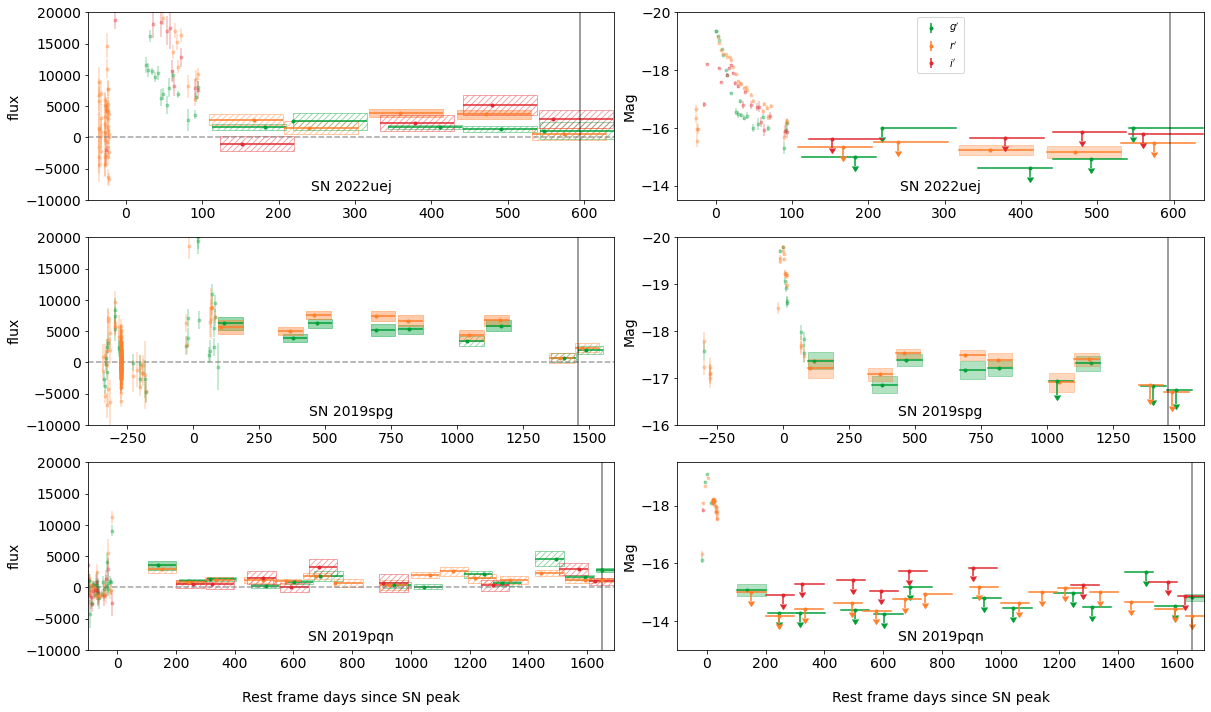
\includegraphics[width=\textwidth]{../Images/chapter_5/non_followup_lcs.png}
    \caption{\textbf{Left:} Binned light curves in flux space in the SN rest frame of the three objects with a late time signal that I could not follow up on. The three ZTF bands \ztfg, \ztfr, and \ztfi\ are shown in green, orange, and red, respectively. Individual observations are shown before the binning starts. Bins are shown as coloured blocks showing the size of the bin, mean value, and $1\sigma$ uncertainty of the binned observations, with the point showing the mean observation date of the bin. Bins that are $>\ 5\sigma$ above zero flux are filled, and bins $\leq5\sigma$ from zero flux are dashed.\\
    \textbf{Right:} Same plot as on the left but in absolute magnitude, corrected for MW extinction. $5\sigma$ detections in individual observations are shown before the binning starts, and the $5\sigma$ binned detections are shown in the same way as in the left plots. $5\sigma$ upper limits are shown with a downward arrow for the binned non-detections. The grey vertical line shows when the excess was first discovered.}
    \label{non_followup_lcs}
\end{figure*}

\textit{\textbf{SN 2019spg.}}
The location of SN 2019spg has a relatively short, sparse baseline before the SN explosion. Immediately after the SN fades, the flux seems to settle at a plateau significantly above the pre-SN baseline. Due to it staying at a nearly constant flux level for much longer than the baseline, this could suggest that the baseline correction was incorrect and the actual baseline should be at the plateau level. With a separation of 0.5$\arcsec$, this object is also very close to the host galaxy nucleus. According to the AGN criterion presented in \citet{WISE_crit}, which uses data gathered with the \textit{Wide-field Infrared Survey Explorer} \citep[WISE,][]{WISE}, the host galaxy is not an AGN. This does, however, not mean that the host cannot show small variability, as has been shown in \citet{Terwel_2024_paper1} and Terwel et al. (submitted). Because of these reasons, I decided not to follow up on this late-time signal. After around 1\,000 days, the flux level dropped again, nearly to the pre-SN baseline level. This drop shows that the previous plateau was a real excess after all, although it was likely related to variability of the host nucleus, not the SN. Due to a combination of unfortunate timing of the excess and unfortunate sampling of the light curve, specifically the pre-SN light curve, these late-time detections of likely nuclear activity looked like a false positive until the signal faded and the original baseline was recovered.

Interestingly, a baseline correction was needed to recover the signal. \textsc{snap} shows no excess in the difference images, but it does show a ghost in the pre-SN region and after the binned signal has faded, which suggests that the excess is in the reference images and that the host dimmed between the time when the reference images were made and the SN explosion.\\


\textit{\textbf{SN 2019pqn.}}
A late-time signal at the position of SN 2019pqn was identified on 28 May 2024, only showing faint \ztfg-band detections that had started 21 days earlier in the rest frame of the SN. This lasted at least 64 days and was active at the end of the monitoring period. Only upper limits in \ztfr- and \ztfi-bands were found at similar epochs. \textsc{snap} shows that the late-time signal lies between the SN and host nucleus locations (which are 1.9$\arcsec$\ apart) but seems to slightly favour the host nucleus location. When this excess was found, I did not have the opportunity to follow it up as I only had very low priority time at the NOT. Therefore, I only have the short period of binned photometry detections. Given that it was only detected in the \ztfg-band, combined with the excess being slightly offset from the SN location, a nuclear transient is a good explanation of this late-time signal, even though the host nucleus is not an AGN according to its WISE colours.


\subsection{Follow-up results}
\label{followups_section}
I found five objects with an active late-time signal for which I could obtain follow-up observations. SN 2019zbq was followed up with the GTC, while the others were followed up with the NOT. Below, I discuss each object individually, starting with the three for which only photometry was taken and then SN 2019zbq, for which I obtained photometry and spectroscopy. SN 2020qxz, for which more extensive follow-up was obtained, is discussed separately in section \ref{sec:SN2020qxz}. The light curves of these objects are shown in Fig.~\ref{followup_lcs}. The details of their follow-up observations are presented in Table \ref{followups}.\\

\begin{figure*}
    \centering
    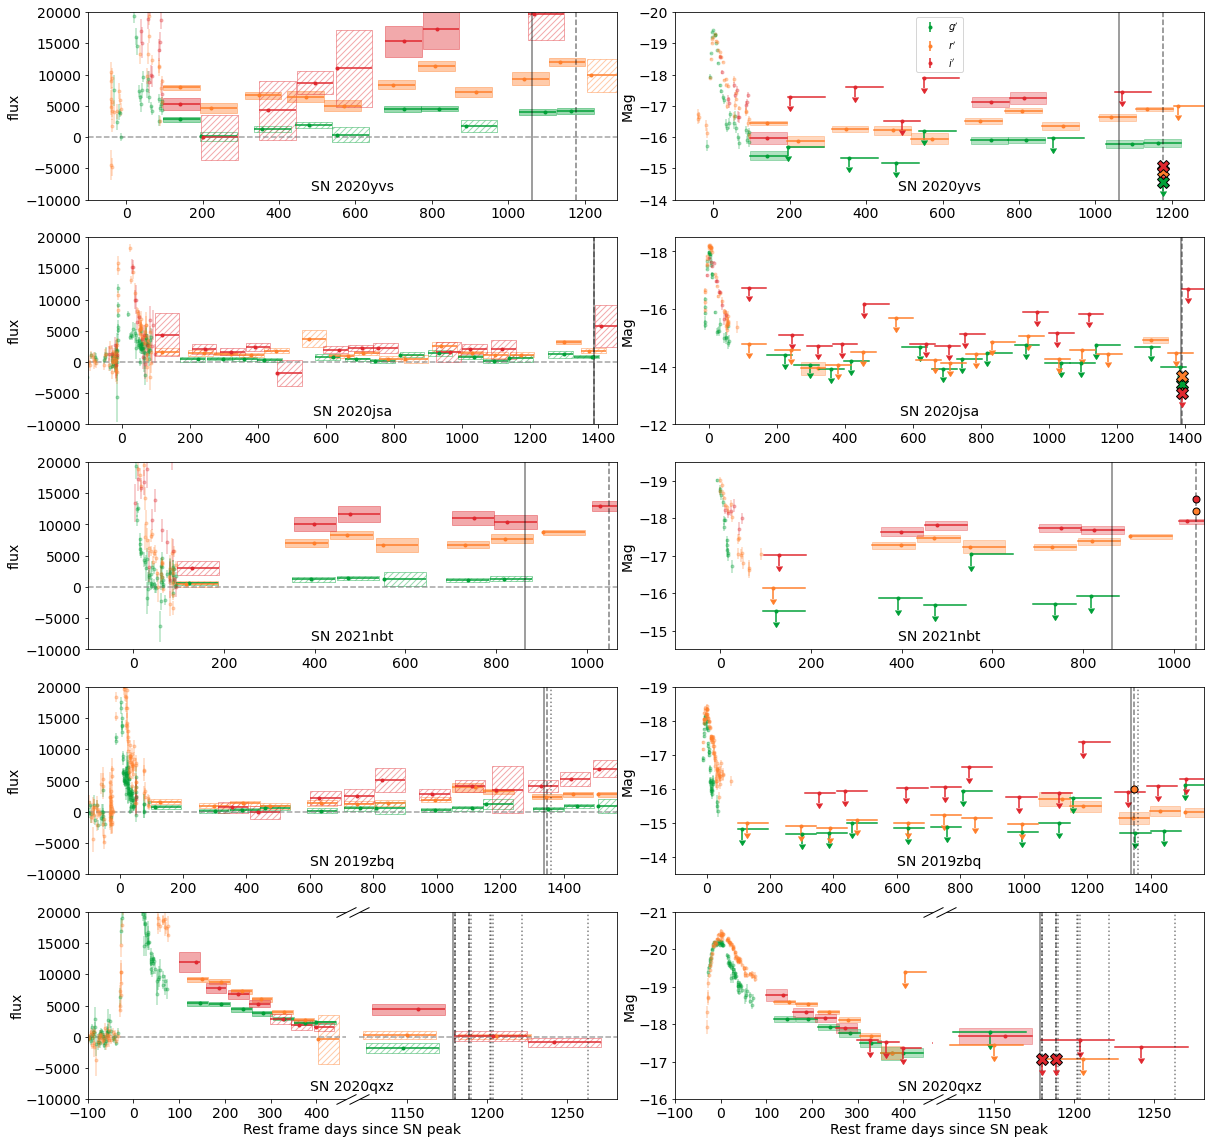
\includegraphics[width=\textwidth]{../Images/chapter_5/followup_lcs.png}
    \caption{Same as Fig.~\ref{non_followup_lcs}, but for the objects for which follow-up observations were made. The grey vertical line shows when the excess was first discovered, and the grey dashed and dotted vertical lines show the photometric and spectroscopic follow-up observations, respectively. The coloured points at the follow-up dates show the follow-up detections and the crosses show the follow-up $5\sigma$ upper limits. Note that for SN 2020qxz the time period between the SN tail and late-time signal has been cut out to better show the detections and follow-up campaign.}
    \label{followup_lcs}
\end{figure*}

\textit{\textbf{SN 2020yvs.}}
On 20 November 2023, SN 2020yvs was found to have elevated flux levels in all three ZTF bands that had started nearly 1\,000 d before, with the effect being stronger in the redder bands. With \textsc{snap} the detected excess is clearly visible, though, at times, it is merged with a residual dipole from the host. As the SN is very close to the bright nucleus of the host galaxy (1.3$\arcsec$, host SDSS \ztfr\ mag = 13.56), I decided to keep a close eye on the development of the light curve to determine if it was more likely to be associated with the SN or not.

As the late-time detections grew stronger over time, I obtained confirmation through photometry with NOT/ALFOSC in the \ztfg\ztfr\ztfi-bands. These observations were obtained on 19 March 2024, with ten exposures of 10 s each using the SDSS \ztfg\ztfr\ztfi\ filters that were stacked together for each band. The short exposures are needed to avoid saturating the host galaxy as image subtraction has to be performed to search for an $\sim 20$ mag excess in an $\sim 13.5$ mag environment. The image subtraction was done through \textsc{autophot} \citep{Autophot} using SDSS images as templates and was attempted using Pan-STARRS images as templates, though these proved to have a saturated host galaxy, making them unusable as templates.

After image subtraction, a small residual at the host nucleus was left, but no excess was found at the SN location. The host residual is the brightest source close to the location, having at most a $2\sigma$ detection at 21.6 mag in the \ztfi-band. This is significantly below the detections found in the late-time ZTF light curve (brighter than mag 20 in both \ztfr\ and \ztfi). Therefore, I conclude that the binned detections are not real but likely due to artefacts in the ZTF images after subtracting the bright host galaxy.\\


\textit{\textbf{SN 2020jsa.}}
The late-time signal in SN 2020jsa was found on 1 May 2024, showing a $21.2\pm0.1$ mag \ztfr-band excess that had begun 112 days earlier and was already fading at the time of discovery. The SN is located 3.0$\arcsec$ from the host galaxy nucleus, and a previous faint detection in the binned late-time light curve can be seen around a year after the SN peak. While the host nucleus is relatively far from the SN, the difference images show a dipole with the positive side towards the SN after host subtraction. This would suggest that there are subtraction issues or that the host shows slight variability. However, according to the WISE criterion, the host galaxy is not an AGN. The object was observed with the NOT in \ztfg\ztfr\ztfi\ the next night, using short exposures to avoid saturation of the bright host and nearby stars. The resulting difference images found no excess at the SN location, providing a deeper limit than the binned ZTF \ztfr-band light curve. However, a faint residual was found at the host nucleus location, showing that the excess is real but unlikely to be related to the SN.\\


\textit{\textbf{SN 2021nbt.}}
The late-time signal in SN 2021nbt was first detected on 5 December 2023. The object is only 0.6$\arcsec$\ from the host nucleus, and its ZTF name is from 2018, which suggests that some host variability caused a first detection long before the SN exploded. This immediately raised suspicion that the detected late-time signal could be related to the host instead. Because of this, it took until 21 June 2024 before I decided to follow it up with the NOT. The signal started relatively shortly after the SN and persisted for several months, which could suggest it is connected to the SN in some way.

After difference imaging was performed on the \ztfr\ztfi-band photometry obtained with the NOT (see Table \ref{followups}), a residual was recovered at \ztfr\ $= 19.458\pm0.040$ mag and \ztfi~$= 19.123\pm0.062$ mag. This is somewhat brighter than the binned detections using ZTF observations taken around the same time, and a signal this bright would have been detectable in the individual ZTF observations. If the host nucleus varies slightly over time, however, this could cause different reference images to show the host at different brightness, which would result in different residuals after difference imaging. Unfortunately, there is no spectrum of the host galaxy, and since the signal is superimposed on the much brighter host, it is impossible to extract a spectrum of the excess without it being completely dominated by the host. The host is too small to attempt extracting a pure host spectrum away from the excess location, and without a host spectrum, the excess contribution cannot be isolated.

At the distance of the host, the magnitude of the excess observed by the NOT translates to an absolute magnitude of M $\sim -18$ mag. As can be seen in Fig.~\ref{followup_lcs}, the excess appears after a gap in the observations and persists for at least 780 days at a fairly constant magnitude. This is at the bright end of the potential ambiguous nuclear transient \citep{2020ohl_Hinkle} population identified in Terwel et al. (submitted), but still consistent with the brightness of the comparison object they use. Due to its shape, brightness, and duration, an ANT that started somewhere between 200 and 400 days after the SN is a good explanation for this excess. However, I do not have spectroscopy to confirm since it was so faint relative to the host.\\


\textit{\textbf{SN 2019zbq.}}
On 13 November 2023, SN 2019zbq was noted to have an active late-time signal in the binned \ztfr-band at m $=21.5\pm0.2$ mag, with the signal already being present for nearly 300 days before and being recovered regardless of bin size or placement. The binned \ztfg-band did not rise from the baseline during this time, but the \ztfi-band did, though the larger uncertainties in this band prevented the detections to reach a $5\sigma$ confidence level. The SN is close to the centre of its host galaxy, with an offset of $1.09\arcsec$.

Checking the \ztfr-band difference images with \textsc{snap} ruled out image defects, reduction or subtraction errors, or a sibling transient with a small sky separation from SN 2019zbq (within the uncertainty of the ZTF resolution) as potential explanations for the detections. The host galaxy has \textit{W1 -- W2} = $0.02\pm 0.04$ and  \textit{W2 -- W3} = $0.9\pm 0.5$, which is not an AGN according to the AGN criterion presented in \citet{WISE_crit}.

\ztfr-band image was obtained with GTC+OSIRIS+ on 23 November 2023. Using \textsc{autophot} and reference images from Pan-STARRS, a m $=20.7\pm0.1$ mag source at the host nucleus location was obtained, which is clearly offset from the SN location, confirming the late-time excess is real but not related to the SN. The GTC image and the resulting difference image are shown in fig.~\ref{2019zbq_difim}.

\begin{figure}
    \centering
    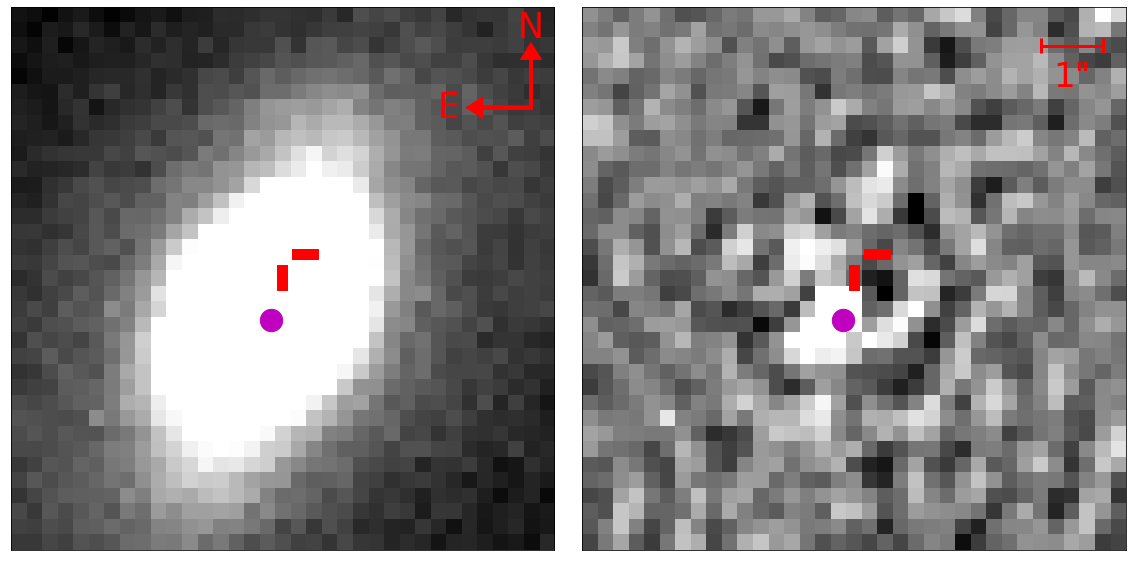
\includegraphics[width=\textwidth]{../Images/chapter_5/2020zbq_difim.png}
    \caption{\textbf{Left:} \ztfr-band image of the location and host galaxy of SN 2019zbq, taken on 23 November 2023 with GTC+OSIRIS+. The SN location is marked in red and the purple dot is the galaxy nucleus location. \textbf{Right:} Difference image of the left region after subtracting a Pan-STARRS template image. There is a residual visible at the host galaxy location. Note that the colour scaling is different for the two images to highlight the important sources.}
    \label{2019zbq_difim}
\end{figure}

On 4 December 2023, a spectrum was obtained with the GTC and OSIRIS+. Since the transient is located on top of the host, this spectrum contains light coming from both the host and the transient. The host is 4.5 mag brighter and dominates the spectrum heavily, meaning the host must be subtracted to recover any potential transient spectrum. Since a slit was used in obtaining the spectrum and the host galaxy is an extended object, A pure host galaxy spectrum is extracted away from the transient location, and I subtract it from the spectrum at the brightest part of the trace containing the transient. Assuming that the spectral features of the host are similar enough at these two locations, the main difference between the two, apart from total flux observed, will be the excess I am interested in.

\begin{figure*}
    \centering
    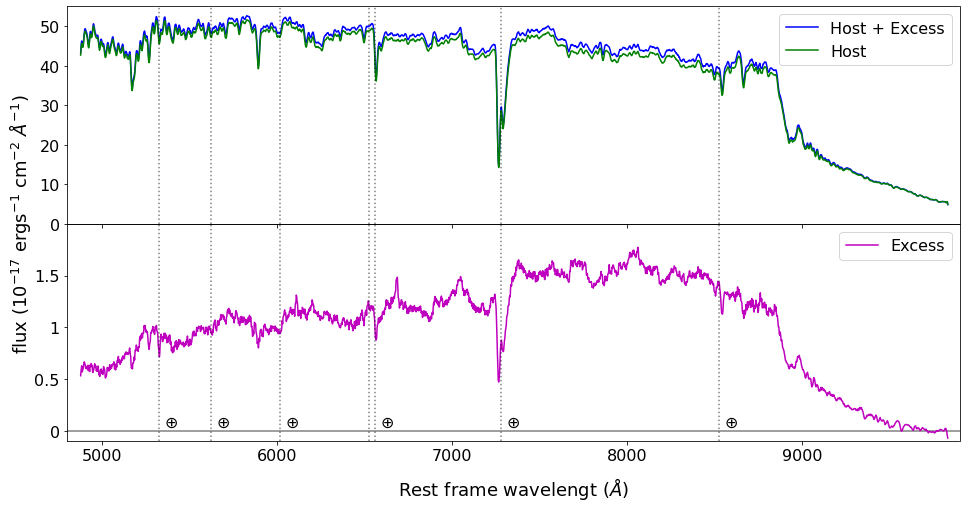
\includegraphics[width=\textwidth]{../Images/chapter_5/2020zbq_spec.png}
    \caption{GTC spectrum of the transient in the SN 2019zbq host galaxy, taken on 4 December 2019. Vertical dotted lines give the locations of sky lines and tellurics. \textbf{Top:} Extracted spectra at the centre of the trace (host + excess) and at the side of the extended host galaxy trace (host). \textbf{Bottom:} The difference of the two spectra in the top panel, showing the isolated spectrum of the excess. The host spectrum has been re-scaled to ensure that the red edge is the same for both spectra.}
    \label{2019zbq_spec}
\end{figure*}

Figure~\ref{2019zbq_spec} shows the extracted host and excess spectra. Since the red edge of the detector has very low sensitivity, this can be used to scale the pure host spectrum to the combined host and excess spectrum, allowing me to take the difference and extract the pure excess spectrum. The pure excess spectrum is shown in the bottom panel. Integrating this spectrum over the \ztfr-band shows this excess to be $\sim21$ mag, which agrees with the photometry values. A few small spikes can be seen in the excess spectrum, but these do not match up with any known emission lines at the host redshift, even when assuming a consistent velocity offset of the excess from the host. Overall, the spectrum looks red, which matches the binned ZTF data, as the \ztfg-band does not rise from zero flux (and the \ztfi-band rises the most but with a large scatter).\\

The excess has an absolute magnitude M $=-16.0$ mag. This, together with the nuclear location and the sudden appearance of the transient followed by a relative stable plateau for over 500 days, is consistent with the faint ANT-like nuclear transients found in Terwel et al. (submitted). Therefore, I conclude that a faint ANT-like transient provides a good explanation for the signal, although I caution that extracting the transient spectrum and removing the host contribution is not straightforward.

\subsection{SN 2020qxz}
SN 2020qxz was classified as a SN Ia-CSM at early times, with a prominent \Halpha\ line visible in the classification spectrum taken around the SN peak, which was used to obtain a redshift of $z=0.0964$ for the object. The slowly decaying tail is visible in the ZTF observations up to 1.2 years after the peak and an additional three months in the binned light curve before fading below the noise limit, resulting in its recovery in \citet{Terwel_2024_paper1}.

On 20 March 2024 (mjd 60389), at nearly 1\,180 d after the SN peak in the rest frame, this object was flagged as currently active due to an elevated flux level in the \ztfi-band in the last four weeks, with the detection being at m $=20.9\pm 0.2$ mag (see bottom row of Fig.~\ref{followup_lcs}). As can be seen in Fig.~\ref{2020qxz_loc}, the SN location is visually offset from the host galaxy, so I obtained follow-up observations with the NOT+ALFOSC on the same night (20 March 2024). The resulting spectrum showed a prominent emission line around $\lambda=9\,210$ \AA\ in the observer frame ($\lambda=8\,400$ \AA\ in the SN rest frame). After this promising detection, I launched a campaign to take more observations (photometry and spectroscopy) with the NOT+ALFOSC over the following weeks.


\subsubsection{Late-time photometry}
Two epochs of \ztfi\ photometry were taken with the NOT+ALFOSC on 20 and 30 March 2024. Both were single 600 s exposures, which were reduced using the method described in section \ref{sec:reduction}. No residual flux above $5\sigma$ was found in either image, resulting in m~=~21.5~mag upper limits. As can be seen in Fig. \ref{followup_lcs}, all observations taken with the NOT were after the detection in the binned ZTF data. However, likely transient flux was detected in the spectra taken at the same epochs as this follow-up photometry. The most likely explanation for the photometric non-detections at the same epochs is that the emission lines seen in the spectra are no longer strong enough to cause a detectable increase in the broadband flux. 

\label{sec:SN2020qxz}
\begin{figure}
    \centering
    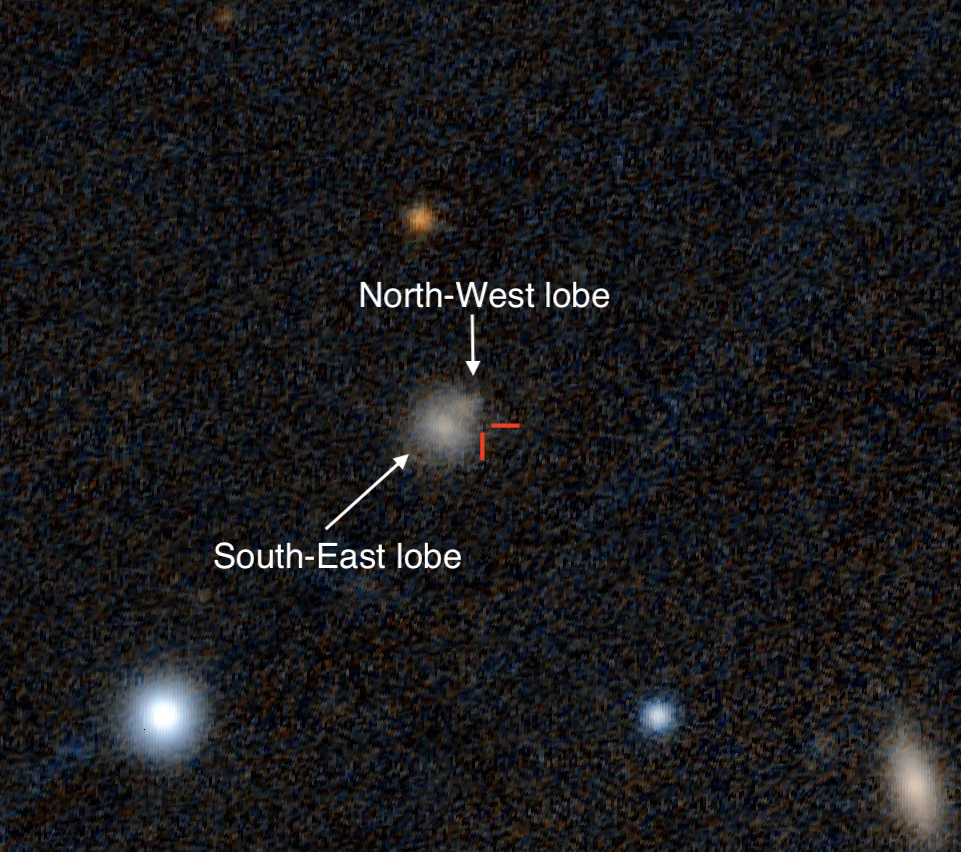
\includegraphics[width=\textwidth]{../Images/chapter_5/2020qxz_loc.png}
    \caption{Pan-STARRS DR1 colour image of the location and host galaxy of SN 2020qxz. The SN location is marked in red, and the two host galaxy lobes are marked in white.}
    \label{2020qxz_loc}
\end{figure}


\subsubsection{Host spectroscopy}
\label{2020qxz_host_specs}
\begin{figure*}
    \centering
    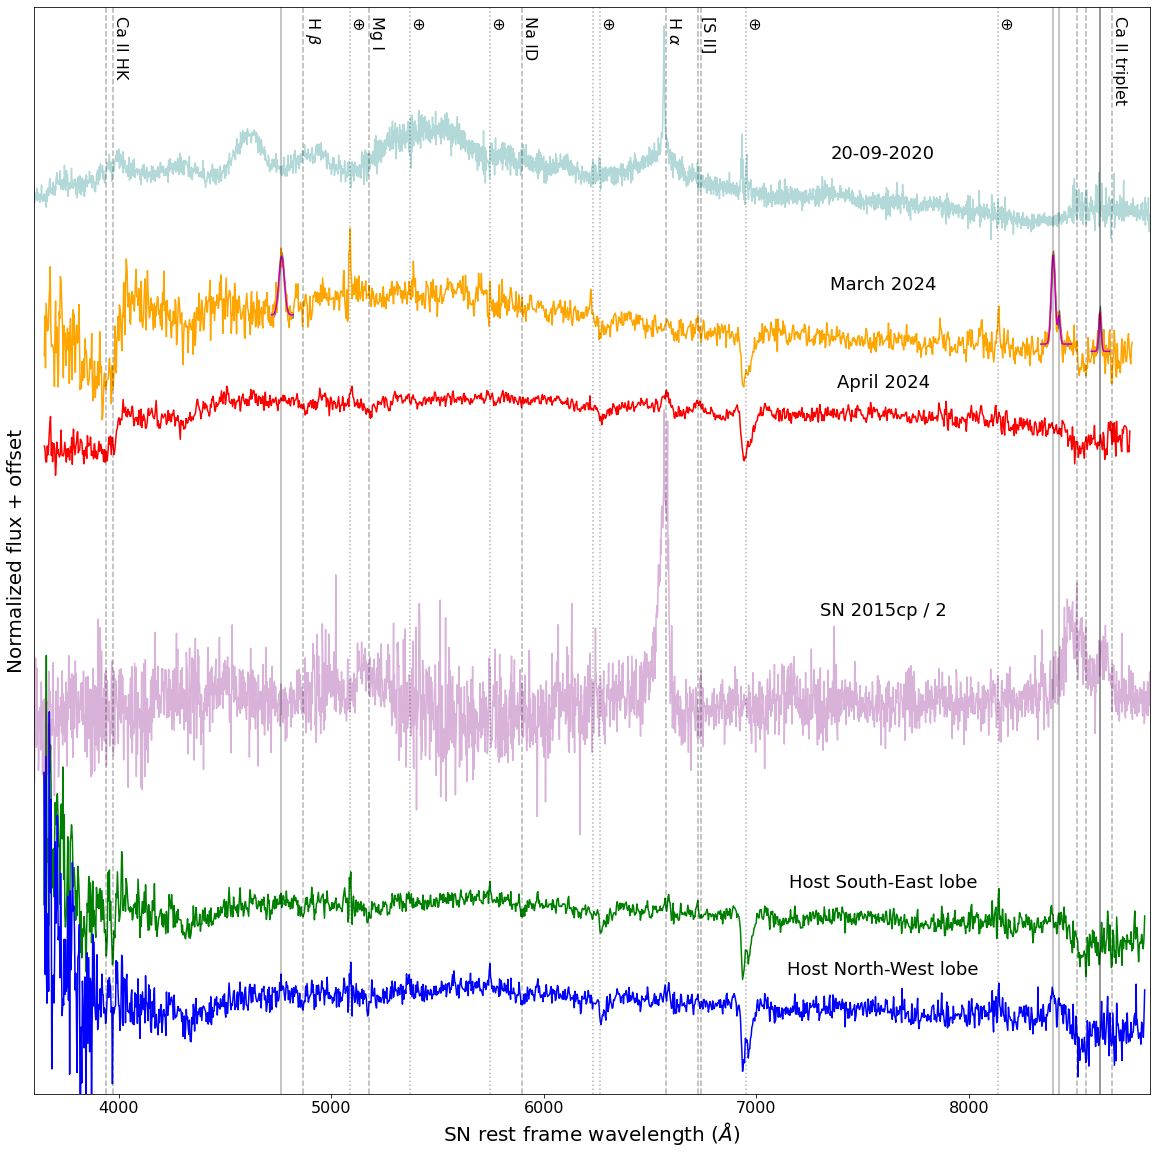
\includegraphics[width=\textwidth]{../Images/chapter_5/2020qxz_spec.png}
    \caption{Combined late-time spectra of 2020qxz and its host in the SN rest frame. The transient emission lines are marked with grey vertical lines, and the best-fit Gaussians are overlaid on top of the combined March spectrum. The dashed vertical lines show the location of host galaxy lines (as well as \Hbeta\ to compare its location to the transient emission line) at the host redshift of $z=0.0975$, and the dotted vertical lines show the location of sky lines. I also show the classification spectrum of SN 2020qzx taken around peak magnitude in light blue and the late-time spectrum obtained for SN 2015cp in magenta, scaled down by a factor of 2 for readability.}
    \label{fig:2020qxz_spec}
\end{figure*}

\begin{figure*}
    \centering
    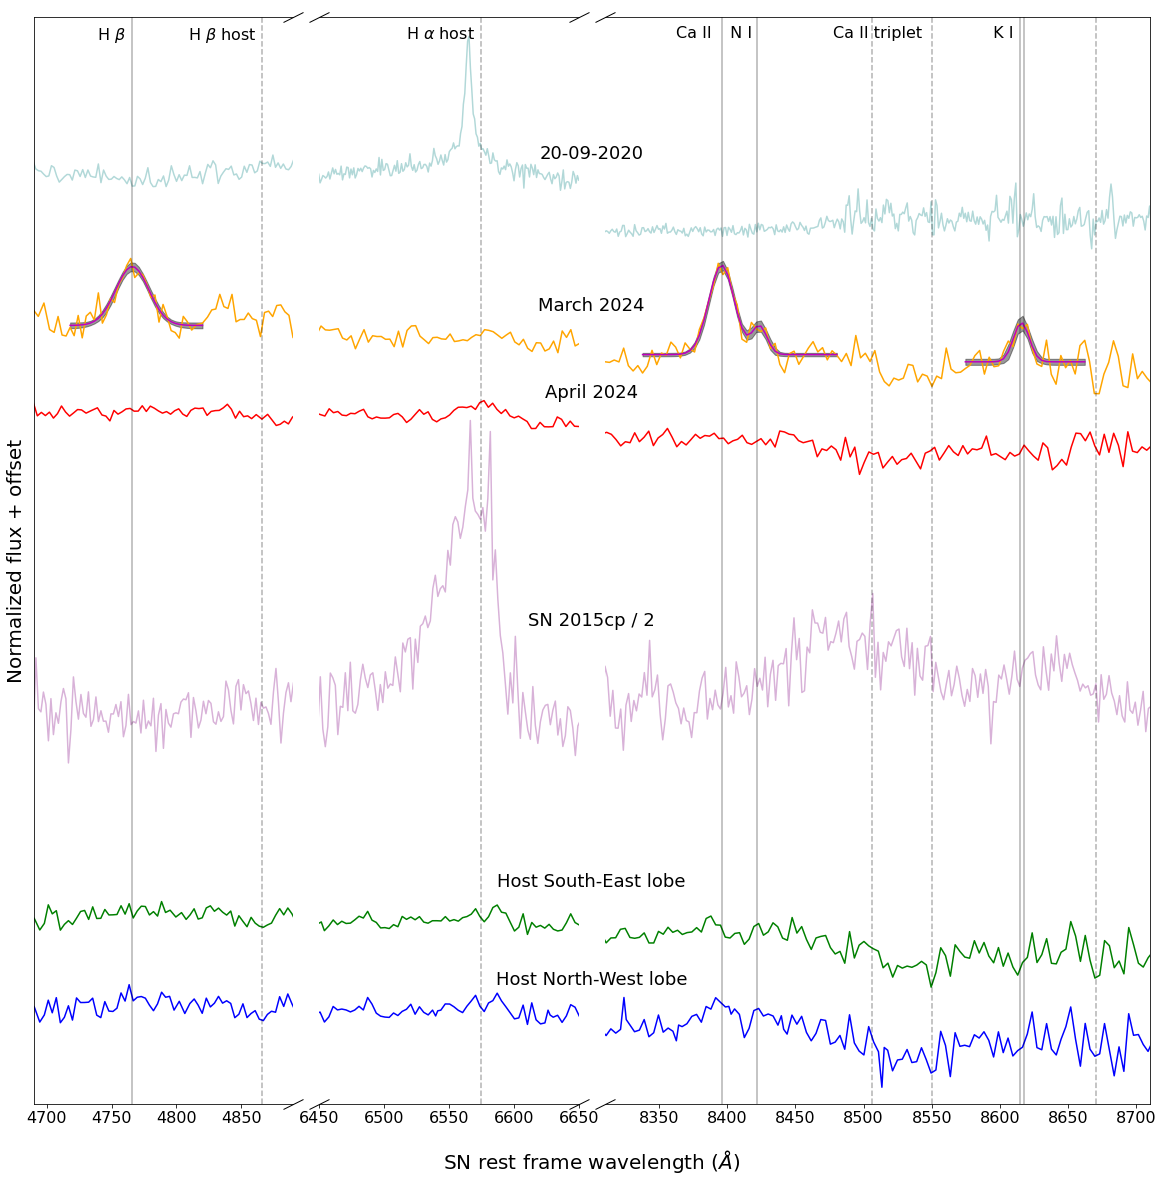
\includegraphics[width=\textwidth]{../Images/chapter_5/2020qxz_spec_zoom.png}
    \caption{Same as Fig~\ref{fig:2020qxz_spec} but zoomed in on the regions containing the transient emission lines and the \Halpha\ region. The $1\sigma$ uncertainties of the Gaussian fits are shown in grey.}
    \label{2020qxz_spec_zoom}
\end{figure*}

The host galaxy of SN 2020qxz has two lobes, a big one on the South-East side and a smaller one on the North-West side (see Fig.~\ref{2020qxz_loc}). By orienting the slit along the axis of the galaxy, I obtained spectra of both lobes on the nights of 3 May and 19 June 2024 with the NOT+ALFOSC, resulting in a two-hour spectrum on the big (South-East) lobe and a one hour and 40 minutes spectrum on the small (North-West) lobe as one of the 20-minute exposures on 3 May 2024 was contaminated at the location of the small lobe and could not be used.

The spectra of the big and small lobes shown at the bottom of Fig.~\ref{fig:2020qxz_spec} look nearly identical, and the galaxy emission and absorption lines discussed below are at the same position for both lobes. This shows that the host is more likely a single object at a single $z$ rather than two distinct galaxies overlapping in the line of sight.

Several lines can be seen in the host spectra. I identify weak lines which I associate with \Halpha\ emission, \SIIF\ emission, \CaII\ H\&K, and NIR triplet absorption, and \NaID\ and \MgI\ absorption. These galaxy lines match the spectrum at $z=0.0975$, which is slightly higher than was found for the \Halpha\ emission seen in the maximum-light classification spectrum of SN 2020qxz as Ia-CSM (top spectrum in Fig.~\ref{fig:2020qxz_spec}). Assuming that the host galaxy is indeed at this higher $z$ and that the SN is associated with the host and at the same $z$, the blueshifted \Halpha\ line in the classification spectrum of SN~2020qxz translates to the SN moving towards us with $\sim200$ km s$^{-1}$ with respect to the host galaxy. The different $z$ value would also slightly change the distance modulus, resulting in all absolute magnitudes being increased by $\sim0.03$ mag. Unless specified otherwise, I use the SN rest frame at $z=0.0964$ while further discussing this object.


\subsubsection{Late-time spectroscopy at the SN location}
\label{2020qxz_spec}
I obtained spectra at several epochs at the position of SN 2020qxz in March and April 2024, which were combined into a `March' spectrum and `April' spectrum (see section \ref{sec:reduction} for further details). In the March spectrum, I identify four prominent emission lines and zero absorption lines that are not associated with the host galaxy. Both the March and April spectra show some signs of slight host contamination, but the four emission lines are only seen in the March data, not in the April spectrum nor the host spectra obtained in May and June 2024. This suggests that these features are transient in nature, and are decaying between the two periods of observations. These emission lines are seen at $4\,766.0\pm1.1$ \AA, $8\,395.8\pm0.6$ \AA,  $8\,423.6\pm1.4$ \AA, and $8\,615.8\pm1.3$ \AA\ in the rest frame of the SN and are marked in Fig.~\ref{fig:2020qxz_spec} and Fig.~\ref{2020qxz_spec_zoom}.

I have fitted these four emission lines with Gaussian profiles to measure their strengths and widths, the results of which are given in Table~\ref{fitres_2020qxz}. The fits to the four lines are shown in Figs.~\ref{fig:2020qxz_spec} and~\ref{2020qxz_spec_zoom}. Three of the lines have a similar dispersion, suggesting that they are from the same source. However, the bluest line has a much higher dispersion that is incompatible with the other three.

\begin{table*}[]
    \centering
    \caption{Line fits for the emission lines identified in the March 2024 spectrum at the position of SN 2020qxz. The first three columns give the central wavelength and width (in \AA\ and km s$^{-1}$) of the fitted lines. The last three columns give the most likely matched elements and emission lines, assuming some amount of blueshift velocity offset (given in the last column). The redshift uncertainty contribution to the velocity offset ($120$~km~s$^{-1}$) has not been included. All fits are done in the SN rest frame.}
    \resizebox{\textwidth}{!}{
    \begin{tabular}{ccc|ccc}
        \hline
        \hline
        Central wavelength (\AA) & $\sigma$ (\AA) & $\sigma$ (km s$^{-1}$) & Element & Rest wavelength (\AA) & Velocity offset (km s$^{-1}$)\\
        \hline
        4\,766.0 $\pm$ 1.1 & 12.7 $\pm$ 1.4 &  800 $\pm$ 88 & \Hbeta & 4\,861.00 & $5\,920\pm70$\\
        8\,395.8 $\pm$ 0.6 & 9.3 $\pm$ 0.7 &  332 $\pm$ 25 & \CaII\ $^{(1)}$ & 8\,542.00 & $5\,180\pm20$\\
        8\,423.6 $\pm$ 1.4 & 5.6 $\pm$ 1.5 &  199 $\pm$ 53 & \NI & 8\,567.74 & $5\,090\pm50$\\
        8\,615.8 $\pm$ 1.3 &5.8 $\pm$ 1.5 & 202 $\pm$ 52 & \KI\ $^{(2)}$ & 8\,763.96, 8\,767.05 & $5\,170\pm50$ \\
        \hline
    \end{tabular}
    }
    \begin{flushleft}
        $^{(1)}$ Only the middle line of the \CaII\ NIR triplet is visible, the other two lines are not present due to atmospheric and host contamination for the blue and red component, respectively.\\
        $^{(2)}$ \KI\ is a doublet for which I use the mean to estimate the velocity offset.
    \end{flushleft}
    \label{fitres_2020qxz}
\end{table*}

Identification of the origin of these emission lines is not straightforward. SN~2020qxz is a known SN Ia-CSM that showed \Halpha\ emission near peak brightness, so it is natural to assume that at least one of the four lines in the March 2024 spectrum is due to H emission. Indeed, the line at $4\,776$ \AA~can be interpreted as \Hbeta\ emission, though this requires it to be blueshifted by $5\,920\pm70$ km s$^{-1}$. Offset emission lines have been found before at up to 10\,000 km s$^{-1}$, see e.g., \cite{2019bkc_Chen} and \cite{2019bkc_Prentice}. However, the significant difference in the hydrogen velocity between the early and late-time detections suggests that this material has been accelerated in the time between detections or is coming from a different location.

SN ejecta sweep up the CSM they are interacting with, so some acceleration can be expected. This has been seen before in some SNe IIn, where aspherical, possibly clumpy CSM has been accelerated to several thousand km s$^{-1}$ resulting in wide boxy or multi-peaked emission lines \citep{1998S_aspherical_CSM, 1998S_late-time, PTF11iqb}. The other issue is that where there is \Hbeta\ emission, one would expect \Halpha\ emission as well. However, there is no sign of any emission line at the position of \Halpha\ in the March or April spectra. There is a small bump that is consistent with being due to host \Halpha\ contamination, but nothing is seen with the same offset as \Hbeta.

The other three transient emission lines at 8\,395.8 \AA,  8\,423.6 \AA, and 8\,615.8 \AA\ in the rest frame of the SN  have their own identification challenges. First of all, these are in the same region as the host galaxy \CaII\ NIR absorption. For the transient emission lines to be visible, this dip in the background spectrum has to be overcome first. Three emission lines are found, but their relative positions are different from the \CaII\ NIR triplet, meaning that not all lines can be explained by them. If I however shift the middle line of this triplet to match with the bluest transient line, the blue line in the \CaII\ NIR triplet overlaps with a skyline while the red line is in the middle of the dip mentioned before. This could explain why only one of the three components is visible. The required blueshift is $5\,180\pm20$ km s$^{-1}$, significantly lower than the shift required for \Hbeta\ of $5\,920$ km s$^{-1}$. A shift of $\sim5\,150$ km s$^{-1}$ allows the remaining two transient lines to be matched to a \NI\ line and \KI\ doublet with the same velocity, resulting in a possible identification of three offset emission lines with similar widths. For the emission line matching with the \KI\ doublet I use the mean wavelength.

Neither of these elements are expected to have a strong presence in the ejecta of SNe Ia, nor have these lines been seen in other SNe with CSM. \citet{2014J_KI} did, however, find time-varying \KI\ absorption lines in SN 2014J around its peak, which they associate with photoionization of distant CSM, although the inferred distance is larger than what the ejecta could travel in a couple of years. It might also be possible to obtain a nitrogen-enhanced CSM if the donor star is an evolved star massive enough to burn hydrogen through the CNO cycle but small enough for the primary to have ended up as a WD. Dredge-ups could bring fusion products to the surface, including nitrogen, which is then lost from the system to form the CSM. \citet{N_lines_SECCSN} make a similar argument for the production of [\NII] lines in stripped envelope CCSNe.

The late-time CSM in SN 2015cp was primarily \Halpha\ dominated \citep{2015cp}, which is absent in SN 2020qxz. At the same time, three of the four emission lines found in SN 2020qxz are absent in SN 2015cp. There is a tentative detection of the \CaII\ NIR triplet in SN 2015cp, but unlike in SN 2020qxz, all three components are observed. They only require a velocity offset of $\sim1\,400$ km s$^{-1}$, though with a FWHM of $\sim3\,000$ km s$^{-1}$ the \CaII\ lines in SN 2015cp are much broader than any of the transient emission lines found in SN 2020qxz.


\section{Discussion}
\label{discussion}
In this study I monitored a sample of 6\,914 SNe Ia discovered by ZTF for signs of late-time rebrightening due to potential CSM interaction. I created forced photometry light curves at the location of each SN for the full duration of the survey and updated these every four weeks with the latest observations in an attempt to find late-time signals in real time and follow them up with further observations. I found 12 objects with late-time rebrightening that could not be explained by image defects, known contamination of host nuclei, or known sibling transients. Four of these were known from \citet{Terwel_2024_paper1} and discussed there. Their rediscovery here did not lead to any new insights. In three objects, the signal was found when follow-up was not possible. I was able to follow the signals in the other five objects up, using the NOT for four objects and the GTC for one. Out of these, there was one false positive, three likely nuclear transients unrelated to the SN, and a confirmed late-time signal in SN 2020qxz.


\subsection{Detection challenges}
As was shown in \citet{Terwel_2024_paper1} and Terwel et al. (submitted), late-time signals in SNe Ia are rare. Out of nearly 7\,000 objects, I found eight objects with a late-time signal detected somewhere in the 240 days as I was actively monitoring them and an additional four objects whose late-time signals were already discussed in \citet{Terwel_2024_paper1}. During this time many other objects were flagged but turned out to be false positives, bright long-lived SNe, or sibling transients. SNe near their host nucleus are especially prone to give false detections.

Most objects for which a late-time signal was flagged in Table~\ref{found_objs}, \citet{Terwel_2024_paper1}, and Terwel et al. (submitted) are close to the host nucleus. These regions are difficult to handle with difference imaging, often leading to residuals that can be mistaken for a weak signal by forced photometry. Even if the excess is real, the busy centres of galaxies leave plenty of opportunity for alternative explanations, including ones involving the central supermassive black hole such as AGN, tidal disruption events and other sources of nuclear variability, e.g. ANTs \citep{2020ohl_Hinkle}. One could make a cut on the host separation to ensure that contamination from nuclear events is removed, but I did not do this here as it would introduce a bias in the SN environments in my sample. Such a cut is also dependent on the pixel size of the used observations, which means that more distant SNe require larger host separations in order to not be removed by the cut. I decided to instead be as inclusive as possible with the knowledge of the contamination this leads to in my results.

Even when searching for faint late-time signals in real time, the fact that my method requires several observations to bin together in order to reach a deeper detection limit results in my method still being slightly behind current events. This makes it crucial to follow up quickly on newly found signals with bigger telescopes and better instruments that are able to measure such faint signals, especially as sometimes the late-time signals have been relatively short-lived and were already fading again by the time they were found. Without my ability to follow up quickly, the transient emission lines in SN~2020qxz might have been missed.


\subsection{Follow-up campaigns}
For five objects that showed late-time signals, I was able to get follow-up photometry, on which difference imaging and forced photometry was performed using \textsc{autophot}. In one case (close to the position of SN 2020yvs), the follow-up observations provided deeper non-detections than the late-time signal that was found in the binned ZTF observations. The host galaxy of SN 2020yvs is very bright, which likely results in small artefacts in the difference images that are misidentified as the late-time signal. In three other cases (close to the positions of SNe 2020jsa, 2021nbt and 2019zbq), a residual was detected at the host nucleus location, showing that for these objects the recovered late-time signal was unrelated to the SN.

The host galaxy of SN 2019zbq was confirmed to have an active nuclear transient and was followed up with spectroscopy. However, since the host galaxy is 4.5 mag brighter than the transient, it dominates the spectrum heavily, and the only way to extract the transient spectrum is by subtracting the host contribution. This requires the existence of a pre-transient host spectrum (from e.g. SDSS, as was done for the late-time signal in SN 2020alm in \citealt{Terwel_2024_paper1}) or a host spectrum without contribution from the transient extracted from the same observation as the spectrum containing the transient, as was done for SN 2019zbq in section~\ref{followups_section}. This is a tricky process and can introduce a lot of uncertainty. For this reason, I did not attempt to get a spectrum of the confirmed excess in the host of SN 2021nbt, as there was already enough evidence of the late-time excess being unrelated to the SN. Integrating the flux of the SN 2019zbq host excess spectrum over the \ztfr-band matches the measured \ztfr-band brightness, showing that the excess extraction has worked.

The excess spectrum in the SN 2019zbq host looks quite red but has no distinctive emission or absorption features. This is similar to the ANT AT 2020ohl \citep{2020ohl_Hinkle}, although AT 2020ohl is much bluer and brighter. The ANTs presented in \citet{wiseman_ztfants} are much closer to the excess in colour but again much brighter, and they all show Balmer emission lines. The small peaks that do stand out in the excess spectrum do not match any set of elements at a single velocity offset. The best I can say about it is that this is indeed some sort of ambiguous nuclear transient.


\subsection{The late-time signal in SN 2020qxz}
\label{2020qzx_discussion}
SN 2020qxz stands out from the other objects in the sample for several reasons. First of all, it is a SN Ia-CSM with detected interaction around its peak. It is also visually separated from its host nucleus, which makes it easier for the excess to be interpreted as being related to the SN instead of nuclear activity, and it is also easier to get a spectrum of the excess without much contribution from the host galaxy. I followed this excess up over three months and obtained nearly six hours of spectroscopic data of the transient, which I combined into a March spectrum and an April spectrum. I also got a spectrum of the two lobes of the host galaxy to confirm that they are not two galaxies overlapping in the line of sight and finding a host redshift of $z=0.0975$. This is slightly higher than the estimated $z=0.0964$ from the \Halpha\ line in the SN peak spectrum, and gives the SN a velocity of $\sim200$ km s$^{-1}$ with respect to the host galaxy. The SN is 3.4$\arcsec$\ from the centre of the South-East lobe, which translates to 7~kpc at the host redshift. This means that the SN velocity can be interpreted as its rotation velocity around the host.

The March spectrum shows four emission lines that are not in the host spectrum, and these had disappeared a few weeks later in the April spectrum. The transient nature of these lines shows that they are associated with the \ztfi-band detection in the binned ZTF light curve. As the follow-up was performed when the late-time signal was already fading again, both the photometric follow-up and the binned observations resulted in non-detection during the follow-up campaign. The remaining transient emission lines are too faint to be picked up in the broadband photometry and are only found during the long spectroscopic observations. This suggests that I only managed to obtain the tail end of the identified signal with spectroscopy.

The only way to match the transient emission lines to elements that can be expected in such an environment is to allow for a large velocity offset. The three lines around 8500 \AA\ all require a velocity of $\sim5\,150$ km s$^{-1}$, matching them with one of the lines of the \CaII\ NIR triplet (the other two are likely contaminated by the host lines, see section \ref{2020qxz_host_specs}), \NI, and \KI\ emission lines. Fitting the lines with Gaussians shows they have similar widths, suggesting that the elements producing these lines are in the same location. The bluest transient line, however, is best matched by \Hbeta\ with an offset of $5\,920\pm70$ km s$^{-1}$. It is also broader than the other three lines. This suggests that, if this line identification is correct, the H-rich material is in a different and faster moving cloud than the N, K, and Ca. It is important to note that although I did not use an order-blocking filter for these observations, none of the emission lines match a second-order diffraction of another emission line, showing that they are four different emission lines.

One problem with the interpretation of the emission line as being \Hbeta\ is that in most cases, when \Hbeta\ is detected, one would also expect to detect \Halpha\ with at least the same strength. This is not the case here, nor is there any sign of an absorption feature at the expected location of \Halpha\ that could completely wipe out a strong, relatively broad emission line like this. However, identifying this line as another element requires a very different velocity and leaves the open question of its strength and width, making \Hbeta\ the best match despite its shortcomings.

The classification of SN 2020qxz as a SN Ia-CSM is due to the \Halpha\ signal around the SN peak from interaction with CSM relatively close to the progenitor system. The late-time signal suggests a second region of CSM further from the progenitor system. Assuming that the inner CSM has a shell or torus-like structure, the interaction signature has the same total redshift as the SN. The late-time transient lines require a significant velocity offset, and their Gaussian profiles were much wider than that of the \Halpha\ line. This shows that the outer CSM is moving much faster and has much more of a patchy structure. Velocity offsets of a few thousand km s$^{-1}$ have been seen before \citep{Maeda_exp_asymetry, Maguire_opt_NIR}. While $>5\,000$ km s$^{-1}$ is high, it is not unprecedented, as the \CaII\ lines in SN 2019bkc have been meaured to be up to $10\,000$ km s$^{-1}$ \citep{2019bkc_Chen, 2019bkc_Prentice}.

CSM with velocity offsets in this regime has been seen before in some SNe IIn. It has been interpreted as material that has been accelerated as it has been swept up. If the CSM is clumpy or disk-like, this can result in a multi-peaked emission line where the redshifted peak is weakened as it comes from the receding end of the SN and has had to travel through dust-forming SN material \citep{1998S_aspherical_CSM, 1998S_late-time, PTF11iqb}. In the case of SN 2020qxz, this could be interpreted as the ejecta running into a shell of H-rich CSM around peak light, resulting in the \Halpha\ line in the classification spectrum. As the CSM is swept up, it is accelerated to at least $\sim6\,000$ km s$^{-1}$ before a part of the accelerated ejecta crashes into a cloud of CSM, resulting in the interaction signal that was observed in 2024. Only the expanding part of the ejecta with accelerated CSM that interacts with this CSM cloud would be emitting light, explaining the offset. However, the viability of such a scenario needs proper modelling.


\section{Conclusions}
\label{conclusion}
In this work I have presented a real-time search of late-time signals in 6\,914 Type Ia SNe in ZTF, using the latest observations to create the most up-to-date light curves for the objects in my sample. By binning the latest observations I was able to go up to nearly one magnitude beyond the single observation limit, which allowed me to find eight new faint signals during the 240-day monitoring effort. Using the NOT and GTC, three of these objects were subsequently followed up with photometry, and two objects were followed up with photometry and spectroscopy. My main conclusions are:

\begin{enumerate}
    \item The requirement to bin observations to get deeper magnitude limits makes even the most real-time strategy lag slightly behind current events. In some cases this resulted in the discovery of a (short-lived) late-time signal while it was already declining again. Quick follow-up is required, but only the tail end of the signal can likely be observed.
    \item Late-time signals are rare, and detections of late-time signals that are associated with the SN are contaminated with detections of associated objects in the same line of sight. This is more prevalent for SNe in or close to the centres of their host galaxies.
    \item In five objects, the late-time detections have been determined to be due to nuclear activity. One of these was not followed up on as it was initially dismissed as a false positive until it faded. This shows the importance of a good baseline when searching for faint signals. The three objects that were followed up showed an excess at the location of the host nucleus, clearly separated from the SN position due to the better resolution.
    \item The excess in the SN 2019zbq host was followed up spectroscopically and showed both similarities and differences to previously studied ANTs, with the main difference being the absolute magnitude of the signal. Since the excess is 4.5 mag fainter than the host nucleus, extracting its spectrum required careful subtraction of the host signal, which complicates studying faint ANTs like these.
    \item The late-time signal in SN 2020qxz stood out from the others, as this is a SN Ia-CSM at $\sim7$ kpc from the host nucleus, making it significantly easier to follow up. While the signal was short-lived, I was able to follow it up spectroscopically, finding four transient emission lines that are best matched by four different elements at two different but highly blueshifted velocities ($5\,150 - 5\,920$ km s$^{-1}$). This suggests that the progenitor system created at least two regions of CSM, one nearby that resulted in the initial Ia-CSM classification and one further away that resulted in the late-time signal.
\end{enumerate}

Faint late-time signals in SNe Ia due to interaction with distant CSM are rare, and even with techniques like binning observations to reach the deepest detection limits, only the brightest and strongest signals can be detected with current surveys. The upcoming Vera C.~Rubin Observatory's Legacy Survey of Space and Time \cite[LSST;][]{LSST} will be able to detect objects several magnitudes deeper than ZTF, allowing the detection of fainter objects in a larger volume. Monitoring existing SN samples like those found by ZTF with LSST will be the best way to find faint late-time signals, which could then be followed up spectroscopically to find the chemical composition of the source of the signal. Constraining the properties of these rare events will allow us to probe the physics that govern SN Ia explosions more thoroughly and gain new insights to help explain them.

\end{document}